\documentclass[12pt,a4paper]{article}

\usepackage{fontspec}  % Latin Modern by default
\usepackage[margin=2.5cm]{geometry}
\usepackage{amsmath,amssymb}
\usepackage{graphicx}
\usepackage{booktabs}
\usepackage{array}
\usepackage{float}
\usepackage{caption}
\usepackage{xcolor}
\usepackage{listings}
\usepackage[colorlinks=true,linkcolor=blue,urlcolor=blue,citecolor=blue]{hyperref}

\captionsetup{labelsep=colon}
\renewcommand{\lstlistingname}{Listing}

\definecolor{codebg}{gray}{0.96}
\definecolor{codeframe}{gray}{0.85}
\definecolor{codecomment}{rgb}{0.0,0.55,0.0}
\definecolor{codenumber}{gray}{0.5}

\lstset{
  language=Python,
  basicstyle=\ttfamily\footnotesize,
  keywordstyle=\color{blue},
  commentstyle=\color{codecomment},
  stringstyle=\color{black},
  numbers=left,
  numberstyle=\tiny\color{codenumber},
  numbersep=6pt,
  backgroundcolor=\color{codebg},
  frame=single,
  rulecolor=\color{codeframe},
  framerule=0.4pt,
  showstringspaces=false,
  breaklines=true,
  tabsize=4,
  columns=fullflexible,
  keepspaces=true,
  captionpos=b,
  xleftmargin=1.5em,
  framexleftmargin=1.5em
}

% partly decrypted text: guessed letters are lower case, the rest is still ciphertext
\newenvironment{cryptotext}{\begin{quote}\raggedright\itshape\small}{\end{quote}}

\begin{document}

% ------------------------------------------------------------------ title page
\begin{titlepage}
  \centering
  \vspace*{0.5cm}
  {\bfseries Ministerul Educaţiei şi Cercetării al Republicii Moldova\par}
  \vspace{0.25cm}
  {\bfseries Universitatea Tehnică a Moldovei\par}
  \vspace{0.25cm}
  {\bfseries Facultatea Calculatoare, Informatică şi Microelectronică\par}

  \vspace{4cm}
  {\LARGE Laboratory work 2:\par}
  \vspace{0.3cm}
  {\Large\bfseries Cryptanalysis of Monoalphabetic Ciphers\par}
  \vspace{0.2cm}
  {\large\bfseries (Frequency Analysis Attack, Variant 16)\par}

  \vspace{3cm}
  \hspace{4cm}
  \begin{minipage}{0.5\textwidth}
    \textbf{Elaborated:}\\
    st. gr. FAF-243 Morari Veaceslav

    \vspace{0.5cm}
    \textbf{Verified:}\\
    asist. univ. Zaica Maia
  \end{minipage}

  \vfill
  {\large Chişinău -- 2026\par}
\end{titlepage}

% ------------------------------------------------------------------ contents
\tableofcontents
\newpage

% ------------------------------------------------------------------ 1
\section{ALGORITHM ANALYSIS}

\subsection{Objective}

Study the frequency analysis attack on monoalphabetic substitution ciphers and apply it
to recover the plaintext and the key of an intercepted English cryptogram (variant 16).

\subsection{Tasks}

An encrypted message was intercepted. It is known that it was obtained with a
monoalphabetic cipher and that the plaintext is written in English. Only the letters were
encrypted; spaces, digits and punctuation were left unchanged. The task is to find the
original message by a frequency analysis attack and to describe the breaking process step
by step, in the same way as in section 2.3 of the laboratory guide. In addition, the key
used for encryption has to be recovered.

\subsection{Theoretical Notes}

A \textbf{monoalphabetic substitution cipher} replaces every plaintext letter with one and
the same ciphertext letter throughout the whole message. The key is a permutation of the
alphabet, so for English there are $26! \approx 4 \cdot 10^{26}$ keys and an exhaustive
search is impossible. The weak point of these ciphers is that they keep the
\textbf{frequency of the letters}: if E is the most common letter in English and it is
encrypted as V, then V will be the most common letter of the ciphertext. The longer the
ciphertext, the closer its letter frequencies are to the general frequencies of the
language (Table~\ref{tab:english}).

\begin{table}[H]
  \centering
  \caption{Frequency of English letters, \% (Table 2.2 of the laboratory guide).}
  \label{tab:english}
  \setlength{\tabcolsep}{3.2pt}
  \small
  \begin{tabular}{l*{13}{c}}
    \toprule
    Letter & A & B & C & D & E & F & G & H & I & J & K & L & M \\
    \%     & 8.17 & 1.49 & 2.78 & 4.25 & 12.70 & 2.23 & 2.01 & 6.09 & 6.97 & 0.15 & 0.77 & 4.03 & 2.41 \\
    \midrule
    Letter & N & O & P & Q & R & S & T & U & V & W & X & Y & Z \\
    \%     & 6.75 & 7.51 & 1.93 & 0.09 & 5.99 & 6.33 & 9.06 & 2.76 & 0.98 & 2.36 & 0.15 & 1.97 & 0.07 \\
    \bottomrule
  \end{tabular}
\end{table}

Frequencies alone rarely give the whole key, because several letters have close
frequencies (for example T, A and O). The analyst also uses other ``personality traits'' of
the language: the most common words (\textit{the}, \textit{and}, \textit{of}, \textit{to},
\textit{a}, \textit{in}), the only one-letter words \textit{a} and \textit{I}, frequent
digraphs (TH, HE, AN, IN, ER) and trigraphs (THE, AND, ING), and partly decrypted words whose
missing letters can be guessed from the context. For this reason the attack is an
interactive process: the computer counts and substitutes, and the human makes the guesses.

% ------------------------------------------------------------------ 2
\section{Introduction}

Frequency analysis is the oldest known cryptanalytic technique. Its first description is
found in the manuscript of Al-Kindi, written around 850 AD. Even today it explains why every
cipher that maps one plaintext symbol to one fixed ciphertext symbol is insecure, no matter
how large its key space is.

\subsection{Intercepted Cryptogram}

The ciphertext of variant 16 contains 3239 letters:

\begin{cryptotext}
Wqv cxipw ngv rtp rtxwxgj xg wqv rxgjp. Wqxp rtp unsf-tsuqtavwxhpdapwxwdwxng, xg wqv cniz nc wqv pwitxjqw-tsuqtavw Kxjvgviv rxwq pqniwivuvtwxgj lvfrnio. Wqv nso naevhwxngp wn xwp dpv, rqxhq anxsvo onrg wnwqv xzunppxaxsxwf nc hniivhwxgj t jtiasvo oxputwhq bdxhlsf vgndjq,ktgxpqvo rxwq wqv wvsvjituq. Xw cdscxssvo wqv ivbdxivzvgwp nc gnghnz-uinzxptaxsxwf nc wqv jvgvits pfpwvz tgo nc vtpv nc lvf hqtgjvp. Znivnkvi,xw qto wqv ivudwtwxng nc avxgj dgaivtltasv---rqxhq, xc xwp hifuwnjitzprviv gnw oxkxovo xgwn rniop, xw stijvsf rtp. Wqv zxsxwtif tonuwvo xw twnghv.Wqvg, xg 1863, t ivwxivo Uidppxtg xgctgwif zteni oxphnkvivo wqvjvgvits pnsdwxng cni wqv uvixnoxh unsftsuqt-avwxh pdapwxwdwxng. Tw ngvpwinlv qv ovznsxpqvo wqv ngsf xzuivjgtasv pwidhwdiv xg hifuwnjituqf.Pxjgts nccxhvip, hnzuvssvo wn uinkxov pvhdiv hnzzdgxhtwxngp, qdgwvocitgwxhtssf cni gvr cxvso hxuqvip. Wqvf cndgo ztgf jnno xovtp xg wqvrixwxgjp nc wqv oxsvwwtgwv hifuwnjituqvip rqn qto uinunpvo hxuqvip cniwqv uinwvhwxng nc uixktwv zvpptjvp. Pnng pnzv nc wqvpv pfpwvzp rvivpvikxgj xg wqv ktixndp tizxvp nc Vdinuv tgo wqv Tzvixhtp. Zniv xovtphtzv cinz tizf nccxhvip rqn qto pwdoxvo hifuwnjituqf xg wqv hndipvp xgpxjgts hnzzdgxhtwxng wqtw wqv gtwxngts zxsxwtif thtovzxvp, pdhq tp Pw.Hfi, qto toovo xg wqv zxo-1800p. Xgvkxwtasf, hifuwtgtsfpwp---rqn rvivvxwqvi tztwvdip ni pnsoxvip rxwq t uincvppxngts xgwvivpw, cni cdssuincvppxngtsp wqviv rviv gngv---ivusxvo rxwq gvr wvhqgxbdvp cni aivtlxgjwqv gvr hxuqvip. Cinz wqv psnr hitrs nc gnzvghstwni otfp, rqvg wqvxgwinodhwxng nc t puvhxts jindu zvtgxgj Oxpivjtio wqv uivhvoxgj jindurndso hngpwxwdwv t ivztiltasv wvhqgxhts toktghv, wqv ithv avwrvvgnccvgpv tgo ovcvgpv xg hifuwnsnjf thhsvitwvo wn xwp znovig uthv.Wqv qxpwnif nc hifuwnsnjf cinz wqv ovhtov wqtw ptr anwq wqv ovtwq ncwqv asthl hqtzavip tgo wqv axiwq nc wqv wvsvjituq wn Rniso Rti X xp wqdpt pwnif nc xgwvigts ovkvsnuzvgw. Rxwqndw Inppxjgnsp ni Rxssvpvp, tgorxwqndw zteni rtip ni oxusnztwxh pwidjjsvp, hifuwnsnjf hndso gnwxgcsdvghv rniso vkvgwp, tgo, vyhvuw cni ngv ni wrn dgdpdts htpvp, xw oxognw. Wqv wvsvjituq stdghqvo wqxp vknsdwxng nc hifuwnsnjf. Xw ainlv wqv zngnunsf nc wqv gnzvghstwni. Wqvgnzvghstwni qto ivxjgvo cni 450 fvtip tp t jvgvits, tss-udiunpv pfpwvz,adw xw hndso gnw zvvw wqv gvr ivbdxivzvgwp vxwqvi nc qxjq-svkvsoxusnztwxh ni zxsxwtif hnzzdgxhtwxngp ni nc snr-svkvs pxjgtshnzzdgxhtwxngp, rqxhq wqv wvsvjituq qto vgjvgovivo. Vthq htssvo cni xwpnrg lxgo nc hifuwnpfpwvz, t puvhxtsxmvo ngv. Pxjgts nccxhvip itglvo wqvpvpfpwvzp xg t qxvitihqf, ixpxgj cinz wqv pxzusv tgo csvyxasv tgo vtpxsfpnskvo wn wqv vywvgpxkv tgo qtio wn pnskv. Wqv wvsvjituq wqdp pwxzdstwvowqv xgkvgwxng nc ztgf gvr hxuqvip tgo, af ivthwxng, ztgf gvr zvwqnopnc hifuw- tgtsfpxp, tgo hnzuvssvo wqvxi tiitgjvzvgw xg t phtsv nchnzusvyxwf.Ztgf nc wqvpv hxuqvip tgo wvhqgxbdvp qtkv avhnzv hstppxh tgo tiv xgdpv wnotf. Znivnkvi, hifuwnjituqf pwxss cdghwxngp wqindjq t qxvitihqftgo vzusnfp t zdswxwdov nc puvhxts pfpwvzp. Wqv wvsvjituq wqvivafcdigxpqvo hifuwnjituqf rxwq wqv pwidhwdiv tgo wqv hngwvgw wqtw xw pwxssqtp. Xw ztov xw rqtw xw xp wnotf. Tss wqvpv wqxgjp qtkv tgwvhvovgwp, tgo edpw tp wqv wvsvjituq xwpvsc oxo,pn rviv wqviv uivhdipnip nc wqv hifuwnjituqxh pfpwvzp wqtw xwvgjvgovivo.Ngv hxuqvi pfpwvz xgkvgwvo avcniv wqv wvsvjituq rtp pn cti tqvto ncxwp wxzv, tgo pn zdhq xg wqv puxixw nc wqv stwvi xgkvgwxngp, wqtw xw ovpvikvpwn av hstppvo rxwq wqvz. Xgovvo, xw ovpvikvp wqv cingw itgl tzngj wqvz,cni wqxp pfpwvz rtp avfngo ondaw wqv znpw ivztiltasv nc tss. Pn rvsshnghvxkvo rtp xw wqtw wnotf, zniv wqtg t hvgwdif tgo t qtsc nc ituxowvhqgnsnjxhts uinjivpp tcwvi xwp xgkvgwxng, xw ivztxgp xg thwxkv dpv.Adw wqvg xw rtp xgkvgwvo af t ivztiltasv ztg, t rvss-lgnrg rixwvi,tjixhdswditsxpw, axasxnuqxsv, tihqxwvhw, oxusnztw, jtojvwvvi, tgo pwtwvpztggtzvo Wqnztp Evccvipng. Qv htssvo xw qxp ``rqvvs hfuqvi,'' tgo xw pvvzpsxlvsf wqtw qv xgkvgwvo xw vxwqvi odixgj 1790 wn 1793 ni odixgj 1797 wn1800.
\end{cryptotext}

\subsection{Tools}

The laboratory guide recommends the online service
\href{https://crypto.interactive-maths.com/frequency-analysis-breaking-the-code.html}{crypto.interactive-maths.com}.
To make every step reproducible, I wrote a small Python program,
\texttt{frequency\_analysis.py}, that does the same work: it counts the letters, compares
them with the English frequencies, applies the guessed substitutions and shows the partly
decrypted text after every guess. As in the guide, the letters that are still encrypted are
shown in UPPER case and the guessed plaintext letters in lower case.

% ------------------------------------------------------------------ 3
\section{IMPLEMENTATION}

\subsection{The Analysis Tool}

\begin{lstlisting}[caption={Counting the letters of the ciphertext}]
def letter_counts(text):
    """Number of occurrences of every letter A-Z (case-insensitive)."""
    counts = Counter(ch for ch in text.upper() if ch in ALPHABET)
    return {letter: counts.get(letter, 0) for letter in ALPHABET}

def sorted_by_frequency(counts):
    return sorted(counts, key=lambda letter: (-counts[letter], letter))
\end{lstlisting}

\texttt{letter\_counts} ignores spaces, digits and punctuation, which were not encrypted,
and counts every letter independently of its case. \texttt{sorted\_by\_frequency} gives the
letters from the most to the least frequent, the order used in Table~\ref{tab:sorted}.

\begin{lstlisting}[caption={Applying the guesses and recovering the key}]
def partial_decrypt(text, mapping):
    result = []
    for ch in text.upper():
        result.append(mapping.get(ch, ch) if ch in ALPHABET else ch)
    return "".join(result)

def add_substitution(mapping, cipher, plain):
    cipher, plain = cipher.upper(), plain.lower()
    for other_cipher, other_plain in mapping.items():
        if other_plain == plain and other_cipher != cipher:
            return f"'{plain}' is already the image of {other_cipher}"
    mapping[cipher] = plain
    return None

def recover_key(mapping):
    inverse = {plain: cipher for cipher, plain in mapping.items()}
    return {plain: inverse.get(plain, "?") for plain in ALPHABET.lower()}
\end{lstlisting}

\texttt{mapping} stores the guesses (ciphertext letter $\rightarrow$ plaintext letter).
\texttt{partial\_decrypt} replaces only the guessed letters, so the analyst sees which
letters are still unknown. \texttt{add\_substitution} rejects a guess that would map two
different ciphertext letters to the same plaintext letter, since a substitution key is a
permutation. \texttt{recover\_key} inverts the mapping to obtain the key in the form of
Table 2.5 of the guide. The program can be used interactively (commands such as
\texttt{V=e W=t}) or can replay all the steps from the file \texttt{variant16\_steps.txt}.

\subsection{Letter Frequencies of the Cryptogram}

The first step is to count all the letters of the cryptogram (Table~\ref{tab:counts}) and
to order them by decreasing frequency (Table~\ref{tab:sorted}).

\begin{table}[H]
  \centering
  \caption{Frequency of the letters in the intercepted cryptogram.}
  \label{tab:counts}
  \setlength{\tabcolsep}{4pt}
  \small
  \begin{tabular}{l*{13}{c}}
    \toprule
    Letter & A & B & C & D & E & F & G & H & I & J & K & L & M \\
    Count  & 38 & 5 & 78 & 72 & 5 & 75 & 203 & 117 & 214 & 67 & 32 & 16 & 1 \\
    \midrule
    Letter & N & O & P & Q & R & S & T & U & V & W & X & Y & Z \\
    Count  & 237 & 130 & 206 & 177 & 58 & 142 & 235 & 83 & 405 & 310 & 239 & 4 & 90 \\
    \bottomrule
  \end{tabular}
\end{table}

\begin{table}[H]
  \centering
  \caption{Letters of the cryptogram in decreasing order of frequency, compared with English.}
  \label{tab:sorted}
  \setlength{\tabcolsep}{3.4pt}
  \small
  \begin{tabular}{l*{13}{c}}
    \toprule
    Ciphertext & V & W & X & N & T & I & P & G & Q & S & O & H & Z \\
    Count & 405 & 310 & 239 & 237 & 235 & 214 & 206 & 203 & 177 & 142 & 130 & 117 & 90 \\
    \% & 12.5 & 9.6 & 7.4 & 7.3 & 7.3 & 6.6 & 6.4 & 6.3 & 5.5 & 4.4 & 4.0 & 3.6 & 2.8 \\
    English & E & T & A & O & I & N & S & H & R & D & L & C & U \\
    \midrule
    Ciphertext & U & C & F & D & J & R & A & K & L & B & E & Y & M \\
    Count & 83 & 78 & 75 & 72 & 67 & 58 & 38 & 32 & 16 & 5 & 5 & 4 & 1 \\
    \% & 2.6 & 2.4 & 2.3 & 2.2 & 2.1 & 1.8 & 1.2 & 1.0 & 0.5 & 0.2 & 0.2 & 0.1 & 0.0 \\
    English & M & W & F & G & Y & P & B & V & K & J & X & Q & Z \\
    \bottomrule
  \end{tabular}
\end{table}

Figures~\ref{fig:english} and~\ref{fig:cipher} show the two distributions. The shapes are
clearly similar, only shifted to other letters, which confirms that a monoalphabetic cipher
was used.

\begin{figure}[H]
  \centering
  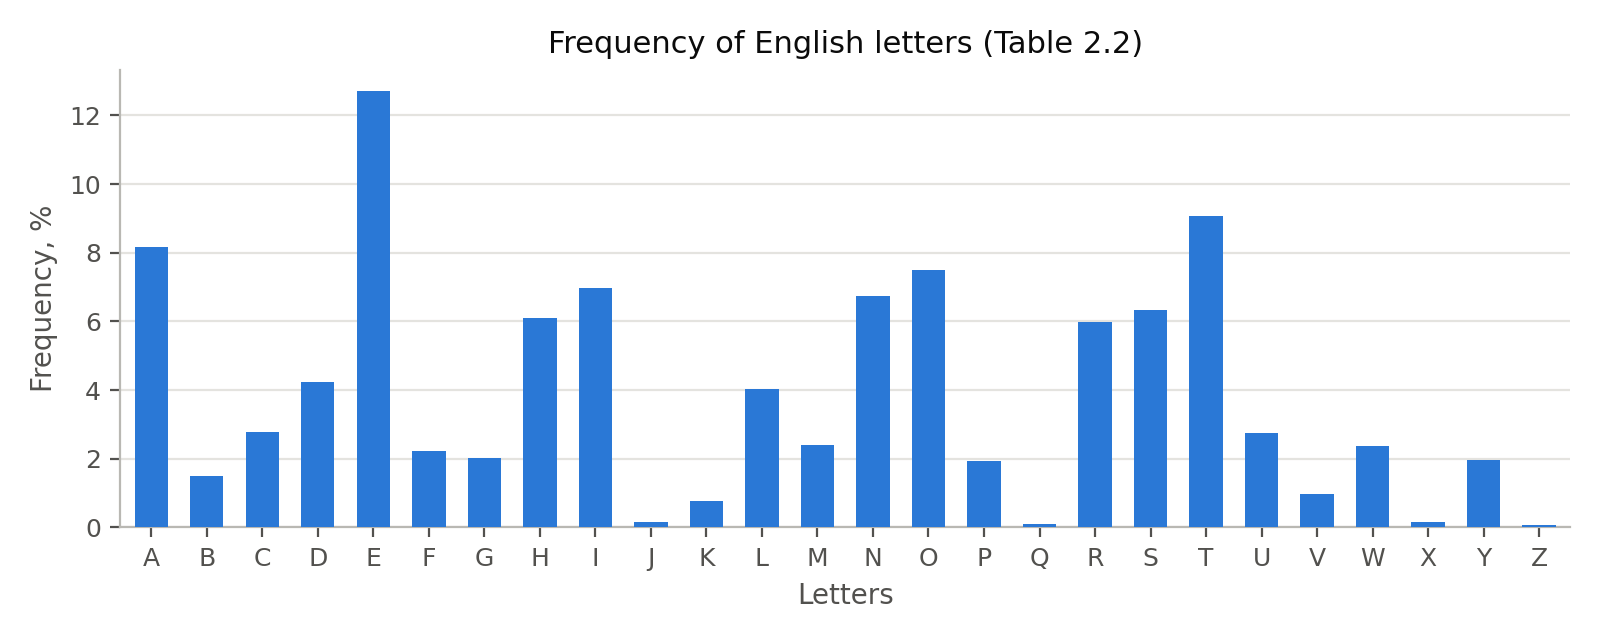
\includegraphics[width=0.9\textwidth]{../charts/english_frequencies.png}
  \caption{Frequency of the letters of the English language.}
  \label{fig:english}
\end{figure}

\begin{figure}[H]
  \centering
  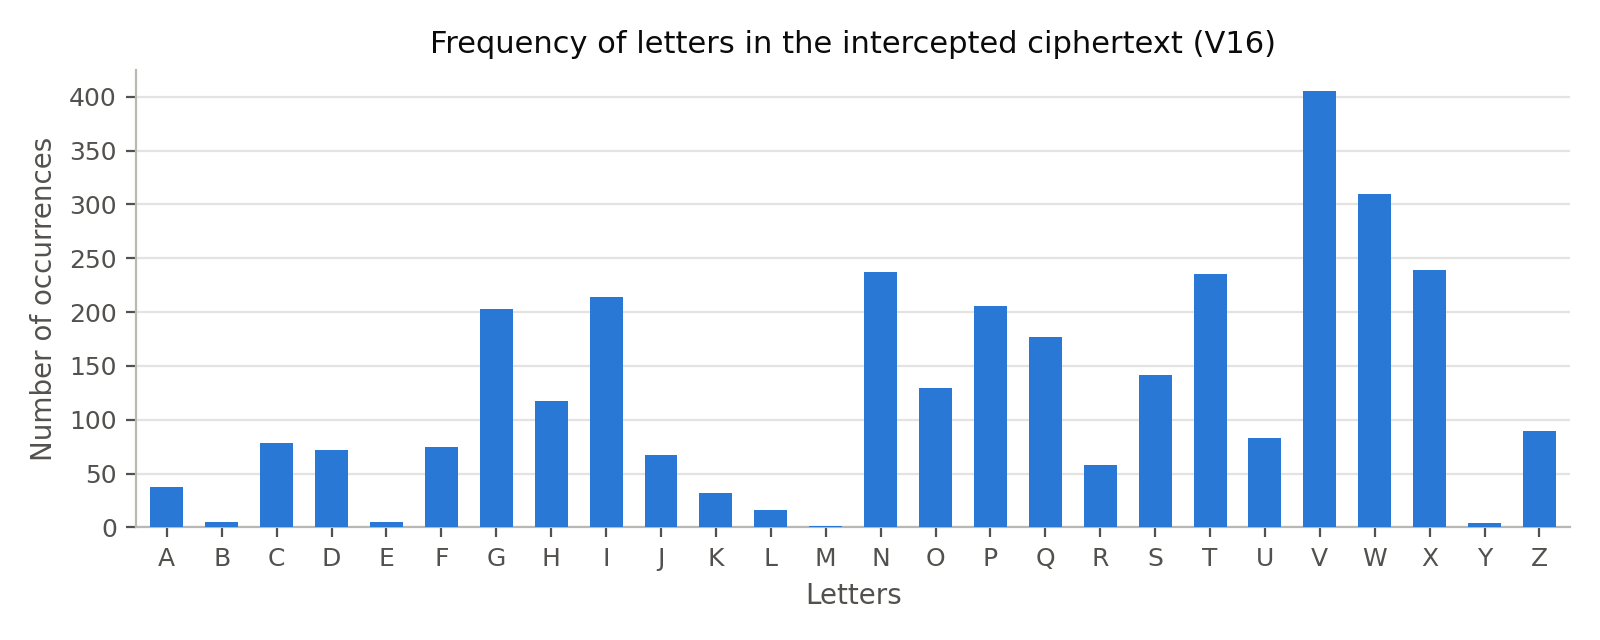
\includegraphics[width=0.9\textwidth]{../charts/ciphertext_frequencies.png}
  \caption{Frequency of the letters in the intercepted cryptogram.}
  \label{fig:cipher}
\end{figure}

\subsection{Breaking the Cipher Step by Step}

To keep the report readable, after every step only the first five sentences of the
cryptogram are shown; the program applies each substitution to the whole text. Lower-case
letters are already decrypted, upper-case letters are still ciphertext. The words that
suggested the next substitution are shown in bold.

\paragraph{Step 1.} The most frequent letter of the cryptogram is V (405 times, 12.5\%),
followed by W (310 times, 9.6\%). In English the two most frequent letters are E (12.70\%)
and T (9.06\%), so we assume V $\rightarrow$ e and W $\rightarrow$ t:

\begin{cryptotext}
\textbf{tQe} CXIPt NGe RTP RTXtXGJ XG tQe RXGJP. tQXP RTP UNSF-TSUQTAetXHPDAPtXtDtXNG, XG tQe CNIZ NC tQe PtITXJQt-TSUQTAet KXJeGeIe RXtQ PQNItIeUeTtXGJ LeFRNIO. tQe NSO NAEeHtXNGP tN XtP DPe, RQXHQ ANXSeO ONRG tNtQe XZUNPPXAXSXtF NC HNIIeHtXGJ T JTIASeO OXPUTtHQ BDXHLSF eGNDJQ,KTGXPQeO RXtQ tQe teSeJITUQ. Xt CDSCXSSeO tQe IeBDXIeZeGtP NC GNGHNZ-UINZXPTAXSXtF NC tQe JeGeITS PFPteZ TGO NC eTPe NC LeF HQTGJeP. ZNIeNKeI,Xt QTO tQe IeUDtTtXNG NC AeXGJ DGAIeTLTASe---RQXHQ, XC XtP HIFUtNJITZPReIe GNt OXKXOeO XGtN RNIOP, Xt STIJeSF RTP.
\end{cryptotext}

\paragraph{Step 2.} The word ``tQe'' appears 44 times, more often than any other word. The
most common three-letter word in English is ``the'', which agrees with the substitutions
already made, so Q $\rightarrow$ h:

\begin{cryptotext}
the CXIPt NGe RTP RTXtXGJ XG the RXGJP. thXP RTP UNSF-TSUhTAetXHPDAPtXtDtXNG, XG the CNIZ NC the PtITXJht-TSUhTAet KXJeGeIe RXth PhNItIeUeTtXGJ LeFRNIO. the NSO NAEeHtXNGP tN XtP DPe, RhXHh ANXSeO ONRG tNthe XZUNPPXAXSXtF NC HNIIeHtXGJ \textbf{T} JTIASeO OXPUTtHh BDXHLSF eGNDJh,KTGXPheO RXth the teSeJITUh. Xt CDSCXSSeO the IeBDXIeZeGtP NC GNGHNZ-UINZXPTAXSXtF NC the JeGeITS PFPteZ \textbf{TGO} NC eTPe NC LeF HhTGJeP. ZNIeNKeI,Xt hTO the IeUDtTtXNG NC AeXGJ DGAIeTLTASe---RhXHh, XC XtP HIFUtNJITZPReIe GNt OXKXOeO XGtN RNIOP, Xt STIJeSF RTP.
\end{cryptotext}

\paragraph{Step 3.} The letter T stands alone as a word 15 times. The only one-letter
English words are ``a'' and ``I'', and T is the fifth most frequent letter, so
T $\rightarrow$ a. The second most frequent word is ``TGO'' (18 times), which with T = a
becomes ``aGO'' and is clearly ``and''. Therefore G $\rightarrow$ n and O $\rightarrow$ d:

\begin{cryptotext}
the CXIPt Nne RaP RaXtXnJ \textbf{Xn} the RXnJP. thXP RaP UNSF-aSUhaAetXHPDAPtXtDtXNn, Xn the CNIZ \textbf{NC} the PtIaXJht-aSUhaAet KXJeneIe RXth PhNItIeUeatXnJ LeFRNId. the NSd NAEeHtXNnP tN XtP DPe, RhXHh ANXSed dNRn tNthe XZUNPPXAXSXtF NC HNIIeHtXnJ a JaIASed dXPUatHh BDXHLSF enNDJh,KanXPhed RXth the teSeJIaUh. \textbf{Xt} CDSCXSSed the IeBDXIeZentP NC nNnHNZ-UINZXPaAXSXtF NC the JeneIaS PFPteZ and NC eaPe NC LeF HhanJeP. ZNIeNKeI,Xt had the IeUDtatXNn NC AeXnJ DnAIeaLaASe---RhXHh, XC XtP HIFUtNJIaZPReIe nNt dXKXded XntN RNIdP, Xt SaIJeSF RaP.
\end{cryptotext}

\paragraph{Step 4.} The two-letter word ``NC'' appears 28 times. The most common two-letter
English word is ``of'', so N $\rightarrow$ o and C $\rightarrow$ f. The words ``Xt'' (19 times)
and ``Xn'' (13 times) can only be ``it'' and ``in'', so X $\rightarrow$ i. The frequencies
agree: N, X and G are among the most frequent ciphertext letters, just like o, i and n in
English:

\begin{cryptotext}
the fiIPt one RaP RaitinJ in the RinJP. thiP RaP UoSF-aSUhaAetiHPDAPtitDtion, in the foIZ of the PtIaiJht-aSUhaAet KiJeneIe Rith PhoItIeUeatinJ LeFRoId. the oSd oAEeHtionP to itP DPe, RhiHh AoiSed doRn tothe iZUoPPiAiSitF of HoIIeHtinJ a JaIASed diPUatHh BDiHLSF enoDJh,KaniPhed Rith the \textbf{teSeJIaUh}. it fDSfiSSed the IeBDiIeZentP of nonHoZ-UIoZiPaAiSitF of the JeneIaS PFPteZ and of eaPe of LeF HhanJeP. ZoIeoKeI,it had the IeUDtation of AeinJ DnAIeaLaASe---RhiHh, if itP HIFUtoJIaZPReIe not diKided into RoIdP, it SaIJeSF RaP.
\end{cryptotext}

\paragraph{Step 5.} The word ``teSeJIaUh'' appears 8 times. The only English word that fits
this pattern is ``telegraph'', which also fits the subject of the text. This gives four
substitutions at once: S $\rightarrow$ l, J $\rightarrow$ g, I $\rightarrow$ r and
U $\rightarrow$ p:

\begin{cryptotext}
the firPt one \textbf{RaP} \textbf{Raiting} in the \textbf{RingP}. thiP RaP polF-alphaAetiHPDAPtitDtion, in the forZ of the Ptraight-alphaAet Kigenere \textbf{Rith} Phortrepeating LeFRord. the old oAEeHtionP to itP DPe, RhiHh Aoiled doRn tothe iZpoPPiAilitF of HorreHting a garAled diPpatHh BDiHLlF enoDgh,KaniPhed Rith the telegraph. it fDlfilled the reBDireZentP of nonHoZ-proZiPaAilitF of the general PFPteZ and of eaPe of LeF HhangeP. ZoreoKer,it had the repDtation of Aeing DnAreaLaAle---RhiHh, if itP HrFptograZPRere not diKided into RordP, it largelF RaP.
\end{cryptotext}

\paragraph{Step 6.} The text now contains ``Rith'' (6 times) and ``Raiting in the RingP'',
which suggest ``with'' and ``waiting in the wings'', so R $\rightarrow$ w. Then ``waP'' (7
times) is ``was'' and ``thiP'' is ``this'', so P $\rightarrow$ s:

\begin{cryptotext}
the first one was waiting in the wings. this was polF-alphaAetiHsDAstitDtion, in the \textbf{forZ} of the straight-alphaAet Kigenere with shortrepeating LeFword. the old oAEeHtions to its Dse, whiHh Aoiled down tothe iZpossiAilitF of HorreHting a garAled dispatHh BDiHLlF enoDgh,Kanished with the telegraph. it fDlfilled the reBDireZents of nonHoZ-proZisaAilitF of the general \textbf{sFsteZ} and of ease of LeF Hhanges. ZoreoKer,it had the repDtation of Aeing DnAreaLaAle---whiHh, if its HrFptograZswere not diKided into words, it largelF was.
\end{cryptotext}

\paragraph{Step 7.} The word ``HrFptographF'' (4 times) is ``cryptography'' and ``HrFptologF''
is ``cryptology'', so H $\rightarrow$ c and F $\rightarrow$ y. Then ``systeZ'' and ``forZ''
are ``system'' and ``form'', so Z $\rightarrow$ m:

\begin{cryptotext}
the first one was waiting in the wings. this was poly-alphaAeticsDAstitDtion, in the form of the straight-alphaAet \textbf{Kigenere} with shortrepeating Leyword. the old oAEections to its \textbf{Dse}, which Aoiled down tothe impossiAility of correcting a \textbf{garAled} dispatch BDicLly enoDgh,\textbf{Kanished} with the telegraph. it fDlfilled the reBDirements of noncom-promisaAility of the general system and of ease of Ley changes. moreoKer,it had the repDtation of Aeing DnAreaLaAle---which, if its cryptogramswere not diKided into words, it largely was.
\end{cryptotext}

\paragraph{Step 8.} Only rare letters are left. ``Dse'' is ``use'' and ``fDlfilled'' is
``fulfilled'', so D $\rightarrow$ u. ``Aeing'' and ``garAled'' give ``being'' and
``garbled'', so A $\rightarrow$ b. ``Kigenere'', ``Kanished'' and ``deKelopment'' are
``Vigenere'', ``vanished'' and ``development'', so K $\rightarrow$ v:

\begin{cryptotext}
the first one was waiting in the wings. this was poly-alphabeticsubstitution, in the form of the straight-alphabet vigenere with shortrepeating Leyword. the old \textbf{obEections} to its use, which boiled down tothe impossibility of correcting a garbled dispatch \textbf{BuicLly} enough,vanished with the telegraph. it fulfilled the \textbf{reBuirements} of noncom-promisability of the general system and of ease of Ley changes. moreover,it had the reputation of being unbreaLable---which, if its cryptogramswere not divided into words, it largely was.
\end{cryptotext}

\paragraph{Step 9.} The last five letters each appear only a few times, and every word
that contains them has only one possible reading: ``BuicLly'' and ``reBuirements'' are
``quickly'' and ``requirements'' (B $\rightarrow$ q, L $\rightarrow$ k); ``Eefferson'' and
``obEections'' are ``Jefferson'' and ``objections'' (E $\rightarrow$ j); ``eYcept'' is
``except'' (Y $\rightarrow$ x); and ``specialiMed'' is ``specialized'' (M $\rightarrow$ z).
Now every letter of the cryptogram is decrypted:

\begin{cryptotext}
the first one was waiting in the wings. this was poly-alphabeticsubstitution, in the form of the straight-alphabet vigenere with shortrepeating keyword. the old objections to its use, which boiled down tothe impossibility of correcting a garbled dispatch quickly enough,vanished with the telegraph. it fulfilled the requirements of noncom-promisability of the general system and of ease of key changes. moreover,it had the reputation of being unbreakable---which, if its cryptogramswere not divided into words, it largely was.
\end{cryptotext}

\subsection{Program Output}

Figures~\ref{fig:run1}--\ref{fig:run3} show the program running in the Windows console.
Figure~\ref{fig:run2} also shows that a wrong guess is rejected: after V $\rightarrow$ e
was fixed, the guess B $\rightarrow$ e is refused, because two ciphertext letters cannot
stand for the same plaintext letter.

\begin{figure}[H]
  \centering
  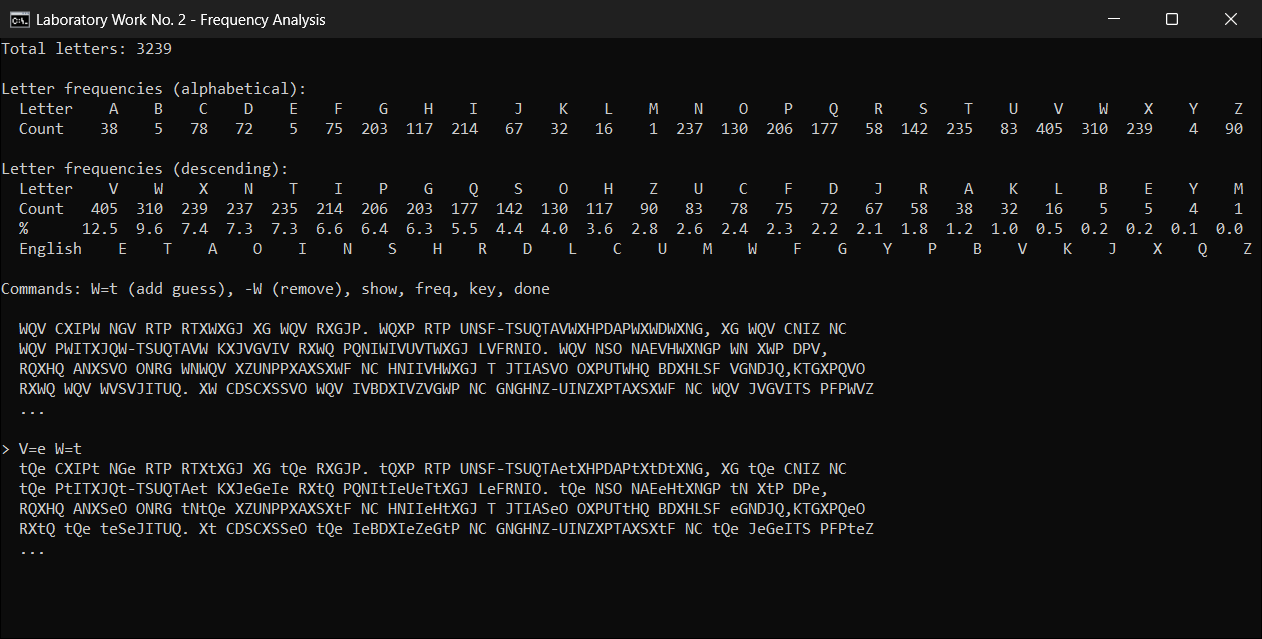
\includegraphics[width=\textwidth]{../screenshots/fig1_frequency_tables.png}
  \caption{Frequency tables of the cryptogram and the first substitution.}
  \label{fig:run1}
\end{figure}

\begin{figure}[H]
  \centering
  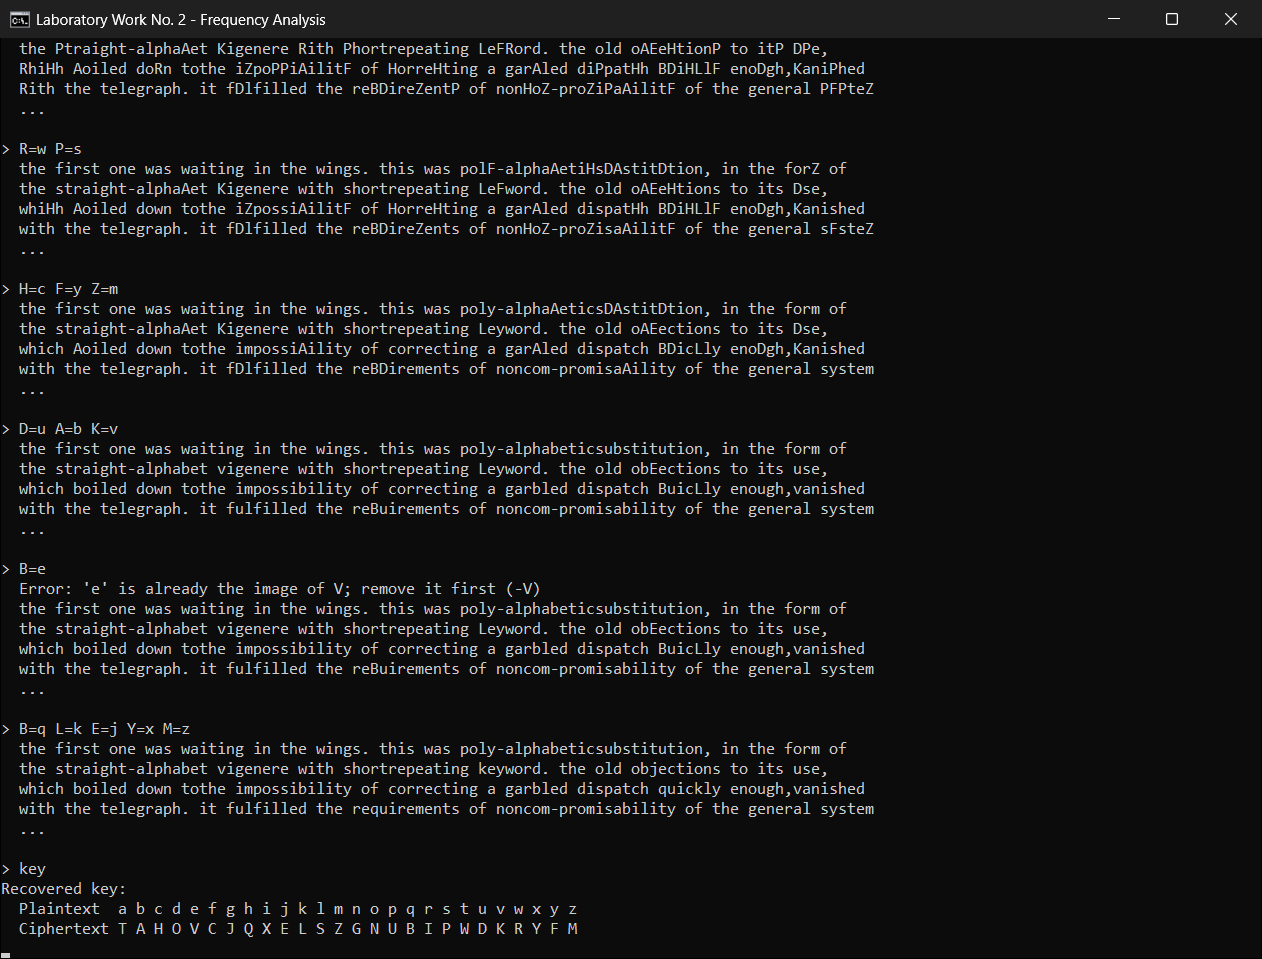
\includegraphics[width=0.95\textwidth]{../screenshots/fig2_substitution_steps_and_key.png}
  \caption{The last substitution steps, a rejected guess and the recovered key.}
  \label{fig:run2}
\end{figure}

\begin{figure}[H]
  \centering
  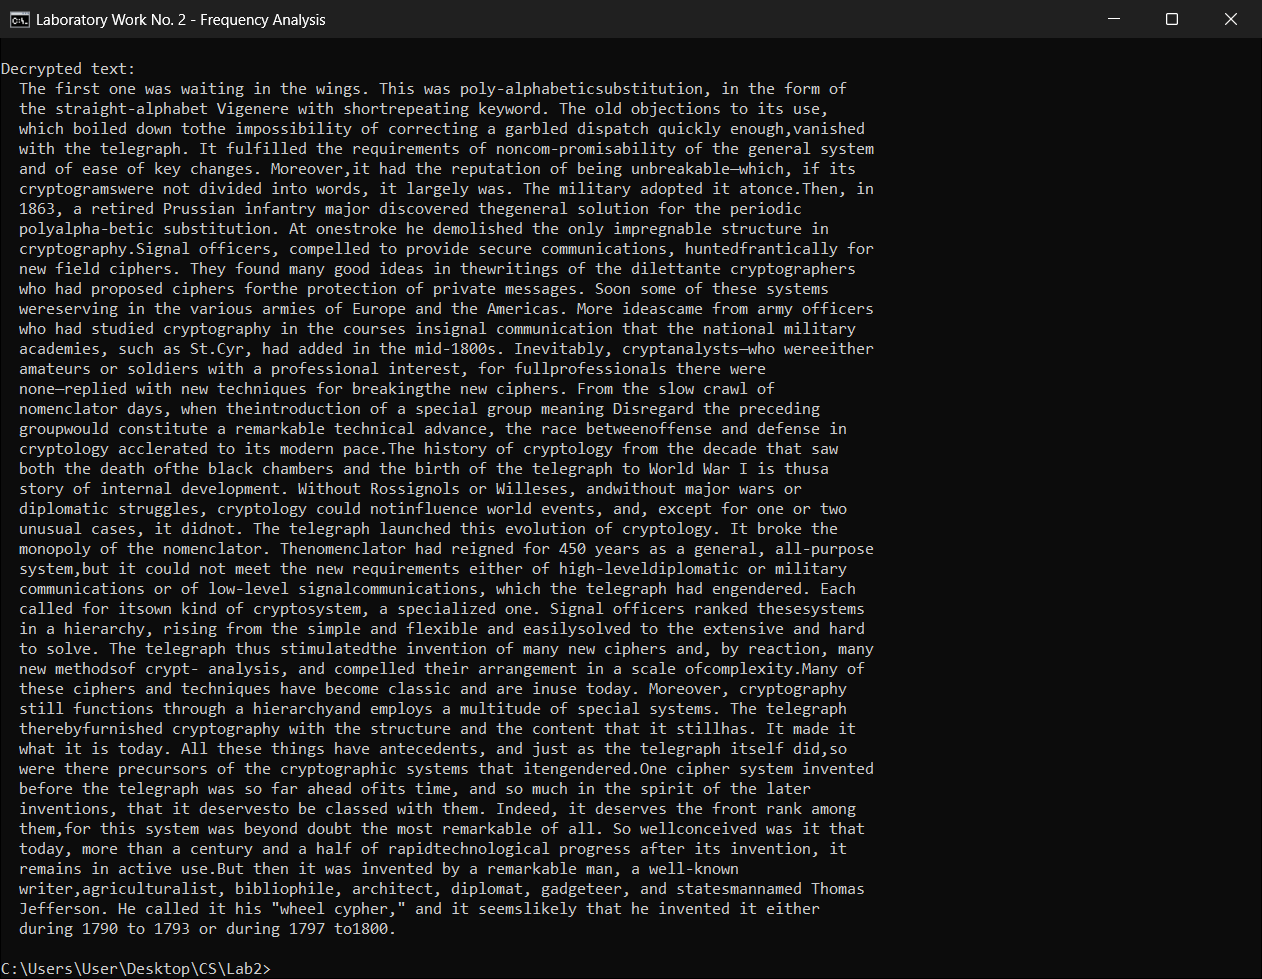
\includegraphics[width=0.95\textwidth]{../screenshots/fig3_decrypted_text.png}
  \caption{The decrypted message.}
  \label{fig:run3}
\end{figure}

\subsection{Results}

The decrypted message (with the original upper and lower case restored) is:

\begin{cryptotext}
The first one was waiting in the wings. This was poly-alphabeticsubstitution, in the form of the straight-alphabet Vigenere with shortrepeating keyword. The old objections to its use, which boiled down tothe impossibility of correcting a garbled dispatch quickly enough,vanished with the telegraph. It fulfilled the requirements of noncom-promisability of the general system and of ease of key changes. Moreover,it had the reputation of being unbreakable---which, if its cryptogramswere not divided into words, it largely was. The military adopted it atonce.Then, in 1863, a retired Prussian infantry major discovered thegeneral solution for the periodic polyalpha-betic substitution. At onestroke he demolished the only impregnable structure in cryptography.Signal officers, compelled to provide secure communications, huntedfrantically for new field ciphers. They found many good ideas in thewritings of the dilettante cryptographers who had proposed ciphers forthe protection of private messages. Soon some of these systems wereserving in the various armies of Europe and the Americas. More ideascame from army officers who had studied cryptography in the courses insignal communication that the national military academies, such as St.Cyr, had added in the mid-1800s. Inevitably, cryptanalysts---who wereeither amateurs or soldiers with a professional interest, for fullprofessionals there were none---replied with new techniques for breakingthe new ciphers. From the slow crawl of nomenclator days, when theintroduction of a special group meaning Disregard the preceding groupwould constitute a remarkable technical advance, the race betweenoffense and defense in cryptology acclerated to its modern pace.The history of cryptology from the decade that saw both the death ofthe black chambers and the birth of the telegraph to World War I is thusa story of internal development. Without Rossignols or Willeses, andwithout major wars or diplomatic struggles, cryptology could notinfluence world events, and, except for one or two unusual cases, it didnot. The telegraph launched this evolution of cryptology. It broke the monopoly of the nomenclator. Thenomenclator had reigned for 450 years as a general, all-purpose system,but it could not meet the new requirements either of high-leveldiplomatic or military communications or of low-level signalcommunications, which the telegraph had engendered. Each called for itsown kind of cryptosystem, a specialized one. Signal officers ranked thesesystems in a hierarchy, rising from the simple and flexible and easilysolved to the extensive and hard to solve. The telegraph thus stimulatedthe invention of many new ciphers and, by reaction, many new methodsof crypt- analysis, and compelled their arrangement in a scale ofcomplexity.Many of these ciphers and techniques have become classic and are inuse today. Moreover, cryptography still functions through a hierarchyand employs a multitude of special systems. The telegraph therebyfurnished cryptography with the structure and the content that it stillhas. It made it what it is today. All these things have antecedents, and just as the telegraph itself did,so were there precursors of the cryptographic systems that itengendered.One cipher system invented before the telegraph was so far ahead ofits time, and so much in the spirit of the later inventions, that it deservesto be classed with them. Indeed, it deserves the front rank among them,for this system was beyond doubt the most remarkable of all. So wellconceived was it that today, more than a century and a half of rapidtechnological progress after its invention, it remains in active use.But then it was invented by a remarkable man, a well-known writer,agriculturalist, bibliophile, architect, diplomat, gadgeteer, and statesmannamed Thomas Jefferson. He called it his ``wheel cypher,'' and it seemslikely that he invented it either during 1790 to 1793 or during 1797 to1800.
\end{cryptotext}

The text is an excerpt about the influence of the telegraph on cryptography and about
Thomas Jefferson's ``wheel cypher''; it appears to come from David Kahn's book
\textit{The Codebreakers}. Words that are joined together, such as ``tothe'' or
``cryptogramswere'', were already joined in the ciphertext.

Placing the plaintext alphabet next to the ciphertext alphabet gives the key that was used
for encryption (Table~\ref{tab:key}). It is useful if other messages from the same sender
are intercepted, since they are likely to use the same key.

\begin{table}[H]
  \centering
  \caption{Reconstructed alphabet of the encrypted message (the key).}
  \label{tab:key}
  \setlength{\tabcolsep}{2.6pt}
  \small
  \begin{tabular}{l*{26}{c}}
    \toprule
    Plaintext & a & b & c & d & e & f & g & h & i & j & k & l & m & n & o & p & q & r & s & t & u & v & w & x & y & z \\
    Ciphertext & T & A & H & O & V & C & J & Q & X & E & L & S & Z & G & N & U & B & I & P & W & D & K & R & Y & F & M \\
    \bottomrule
  \end{tabular}
\end{table}

% ------------------------------------------------------------------ 4
\section{CONCLUSION}

Within this laboratory work, a monoalphabetic substitution cipher was broken by a frequency
analysis attack, without any knowledge of the key. The intercepted cryptogram of variant 16
(3239 letters) was fully decrypted in nine steps, and the whole key, a permutation of the 26
English letters, was recovered.

\textbf{Letter frequencies give the first foothold.} The two most frequent ciphertext
letters, V (12.5\%) and W (9.6\%), matched E (12.70\%) and T (9.06\%) exactly. For the
following letters the frequencies alone were not enough: X, N, T, I, P and G all have
frequencies between 6.3\% and 7.4\%, so their order did not match the English order A, O, I,
N, S, H. Frequencies only narrowed the choice; the final decision came from the words.

\textbf{The structure of the language does the rest.} The most useful clues were the
frequent short words (``the'', ``and'', ``of'', ``a'', ``it'', ``in'') and long words with a
unique pattern, such as ``telegraph'' and ``cryptography'', which gave four letters at once.
After about half of the letters were known, the remaining ones followed almost
automatically from the context. The rarest letters (J, Q, X, Z) could only be found this
way, because they appear just a few times.

\textbf{Monoalphabetic ciphers are insecure regardless of the size of their key space.}
Although there are $26! \approx 4 \cdot 10^{26}$ possible keys, a text of a few thousand
letters was broken in a few steps, because the cipher preserves the statistics of the
language. The attack would be harder for a very short message, for a text without spaces
between the words, or for a polyalphabetic cipher such as the Vigen\`ere cipher, which is
the subject of the decrypted text itself.

In conclusion, during this work I learned how to perform a frequency analysis attack, how to
combine statistics with the knowledge of the language, and how to automate the routine part
of the work with a small program, while the guesses are still made by the analyst.

\section{SOURCE CODE}

The full source code is available on GitHub:
\url{https://github.com/veacheslavv/CS_Labs/tree/main/Lab2}

\end{document}
